\documentclass[main.tex]{subfiles}
%\documentclass[14pt,a4paper,twoside]{extarticle}	% Размер основного шрифта и формата листа
%\usepackage{xltxtra,xunicode,polyglossia}						% Используется для вывода логотипа XeLaTeX
%\newfontfamily\russianfont{Liberation Serif}
%\usepackage{standalone}
%\usepackage{tikz}
%\setdefaultlanguage{russian}				% Основной язык текста
%\setotherlanguage{english}					% Дополнительный язык текста
%\linespread{1}							% Межстрочный интервал выбран полуторным
%\usepackage[left=2.5cm,right=1.5cm,vmargin=2.5cm]{geometry} % Отступы по краям листа
%
%\usepackage{xcolor,hyperref}
%\definecolor{linkcolor}{HTML}{359B08} % цвет ссылок
%\definecolor{urlcolor}{HTML}{799B03} % цвет гиперссылок
%\hypersetup{pdfstartview=FitH,  linkcolor=linkcolor,urlcolor=urlcolor, colorlinks=true}
%
%\usepackage{verbatim,indentfirst,cite,enumerate,float,amsmath,amssymb,amsthm,amsfonts}
%\usepackage{graphicx,fontspec,subfigure}

\begin{document}
%\pagestyle{empty} %  выключаенм нумерацию
%\setcounter{page}{3}% Нумерация начинается с третьей страницы
%\renewcommand{\contentsname}{\center{Содержание}}
%\tableofcontents

\begin{center}
	%\addcontentsline{toc}{section}{Опыт 7. Сложение движений}
	\subsection*{Сложение движений}
\end{center}

\begin{figure}[H]
	\centering 	
	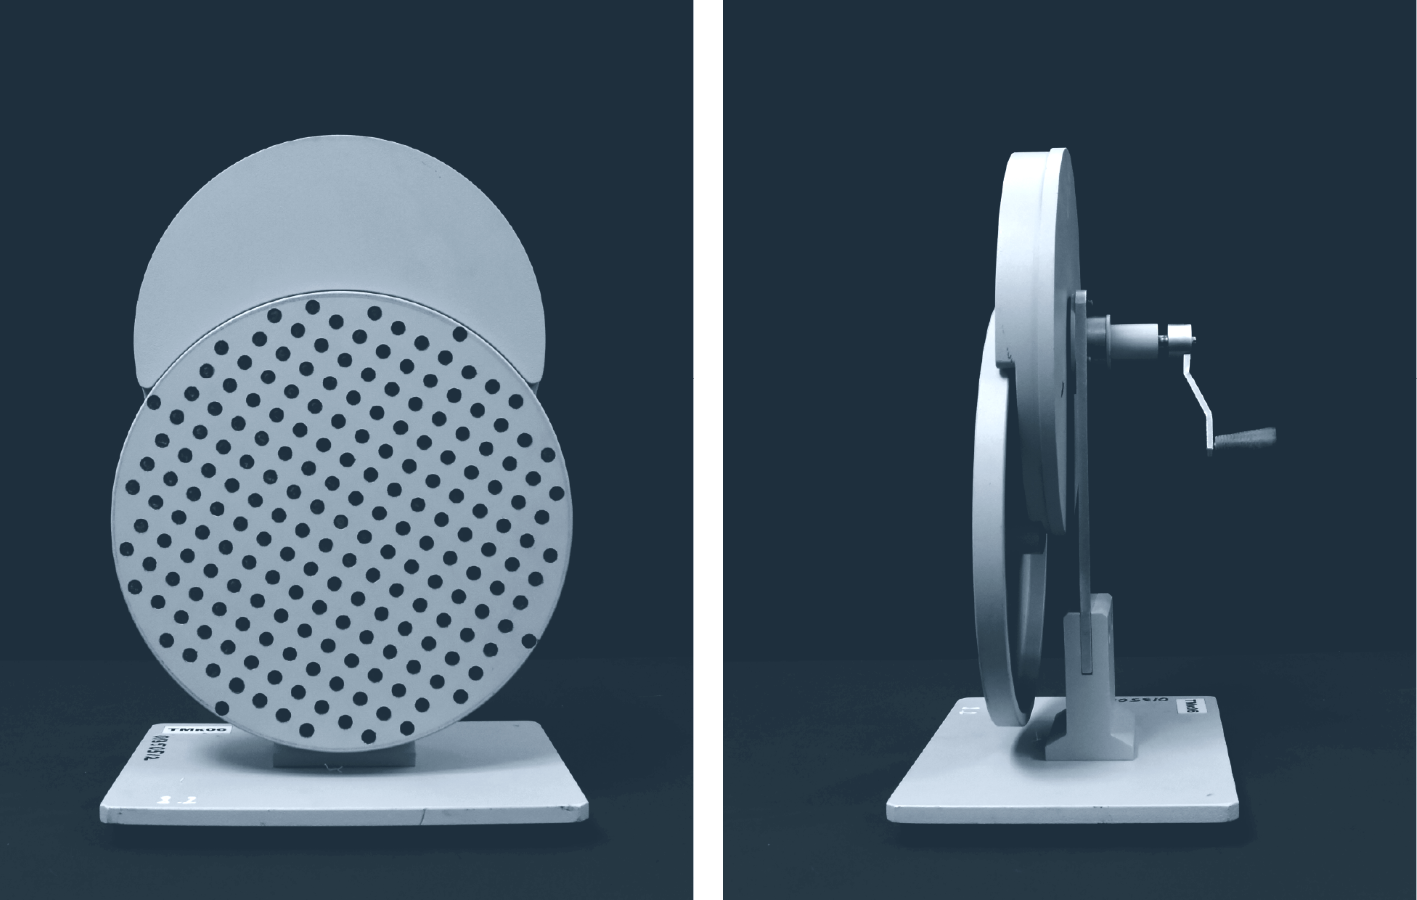
\includegraphics[width=0.8\linewidth]{aom-1.png}
	\caption{Демонстрация сложения параллельных вращений}
	\label{aom-1}
\end{figure}

\subsection*{\underline{Оборудование:}}

\begin{enumerate}
	\item Диск диаметром 26 см, поверхность которого покрыта темными кружками диаметром 1 см.
	\item Подставка с механизмом, приводящим диск во вращение как вокруг его собственной горизонтальной оси, так и в вертикальной плоскости его движения.
\end{enumerate}

\subsection*{\underline{Основные определения:}}

Вообще говоря, при движении твердого тела разные точки движутся по различным траекториям с различными скоростями.
Но оказывается, что всегда можно произвольное движение твердого тела представить как сумму  независимых движений: поступательного и вращательного.

\textit{\begin{flushleft}
Поступательным движением твердого тела называется такое движение, при 
котором любая прямая, проведенная в теле, остается параллельной 
самой себе. 
При поступательном движении все точки тела движутся одинаково. 
\end{flushleft}}

\textit{\begin{flushleft}
Вращательным движением твердого тела называется такое движение, при котором все точки тела движутся по концентрическим окружностям, а все центры этих окружностей лежат на одной прямой, называемой осью вращения.
\end{flushleft}}

\subsection*{\underline{Краткое описание:}}

Закрепленный на подставке диск обладает горизонтальной осью вращения, проходящей через его центр.
При этом вращательный механизм способен приводить в движение по окружности и саму ось.

Раскрутив изначально неподвижный диск вокруг собственной оси, можно наблюдать вращение темных кружков.
Удаленные от центра пятна при быстром вращении начнут сливаться в линии, а кружок в центре диска, лежащий на оси вращения, останется неподвижным (рис.\ref{aom-2}).

\begin{figure}[H] 
	\centering 	
	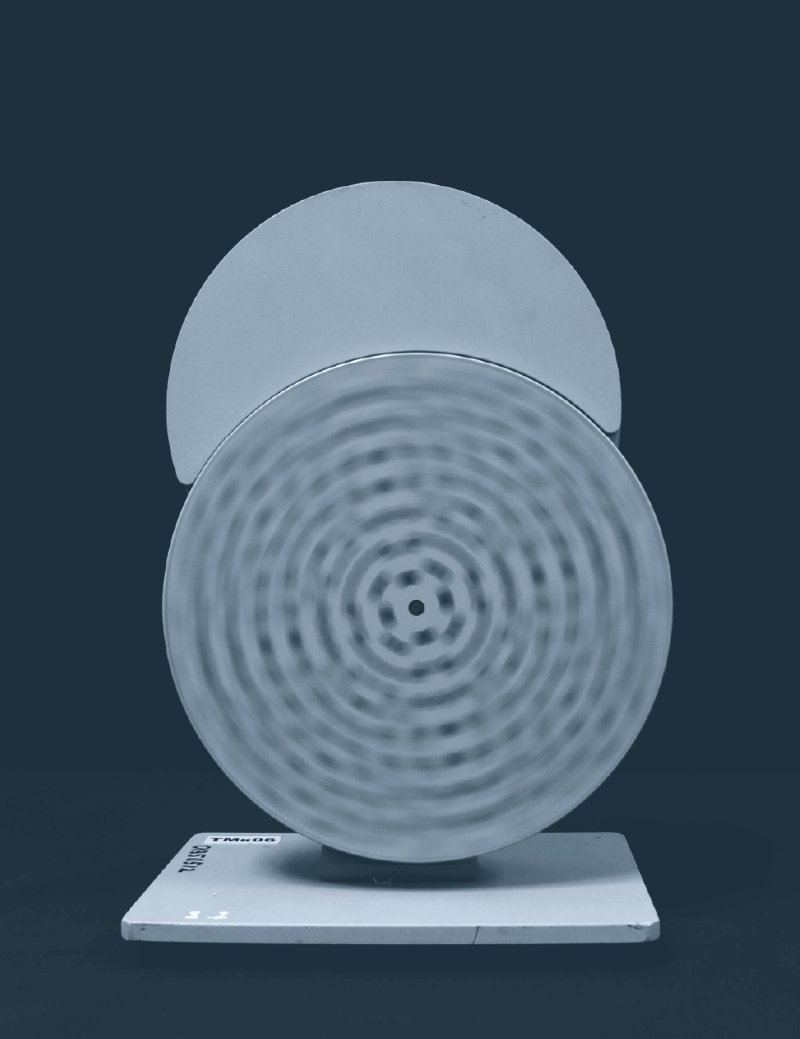
\includegraphics[width=0.35\linewidth]{aom-2.png}
	\caption{Вращение диска вокруг собственной оси, проходящей через его центр}
	\label{aom-2}
\end{figure}

Если при вращении диска его центральная ось начнет двигаться оп окружности в вертикальной плоскости, параллельной диску (рис.\ref{aom-3}), то результирующее движение можно описать как вращение вокруг мгновенной оси, которая совершает круговое движение. В каждый момент времени мгновенная ось вращения твердого тела оказывается в новом положении, которое можно обнаружить по положению кружка, кажущегося неподвижным. Этот неразмытый кружок не совпадает с центром диска, а перемещается по окружности в вертикальной плоскости.

\begin{figure}[H]
	\centering 	
	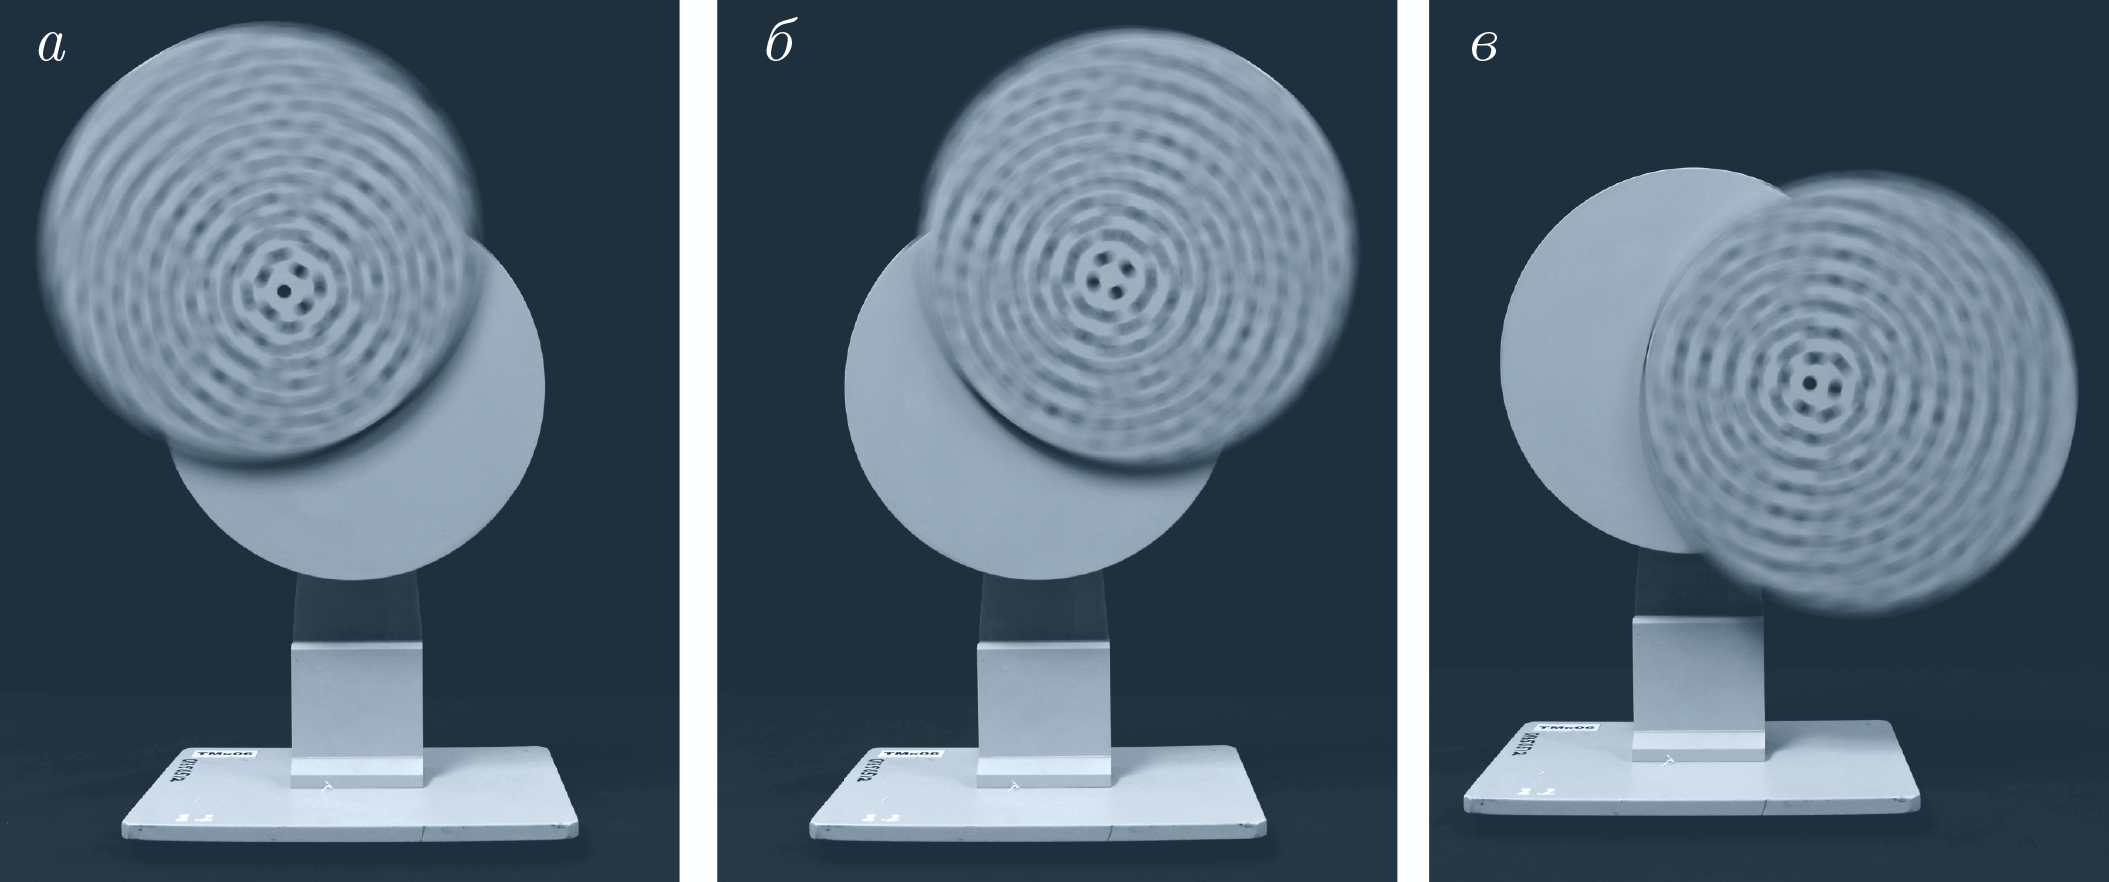
\includegraphics[width=0.9\linewidth]{aom-3.png}
	\caption{Четкое пятно находится не в центре, что связано с появлением новой — мгновенной оси вращения. Вращение диска вокруг мгновенной оси возникает в результате наложения движения диска вокруг собственной ось и перемещении оси вращения по окружности}
	\label{aom-3}
\end{figure}

\subsection*{\underline{Теория:}}

Пусть диск вращается против хода часовой стрелки.
Обозначим угловую скорость его вращения через $ \textbf{ω}_1 $ (рис.\ref{aom-4},\textit{б}).

\begin{figure}[H] 
	\centering 	
	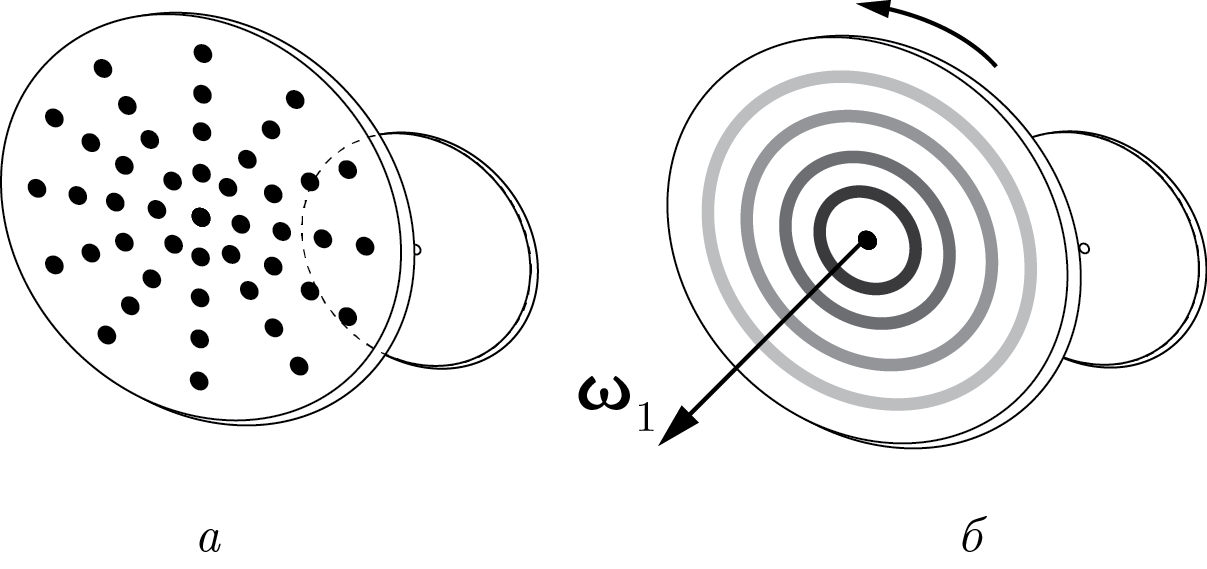
\includegraphics[width=0.6\linewidth]{aom-4.png}
	\caption{\textit{а} — схематичное изображение неподвижного диска на штативе; \textit{б} — направление вектора угловой скорости диска при его вращении против хода часовой стрелки}
	\label{aom-4}
\end{figure}

Так как ось диска жестко связана с валом на штативе, то при вращении вала (рис.\ref{aom-5}\textit{а}) с угловой скоростью $ \textbf{ω}_2 $, результирующая угловая скорость вращения диска $\textbf{ω}$ равна векторной сумме скоростей диска и вала: $\textbf{ω} = \textbf{ω}_1 + \textbf{ω}_2$.

\begin{figure}
	\centering 	
	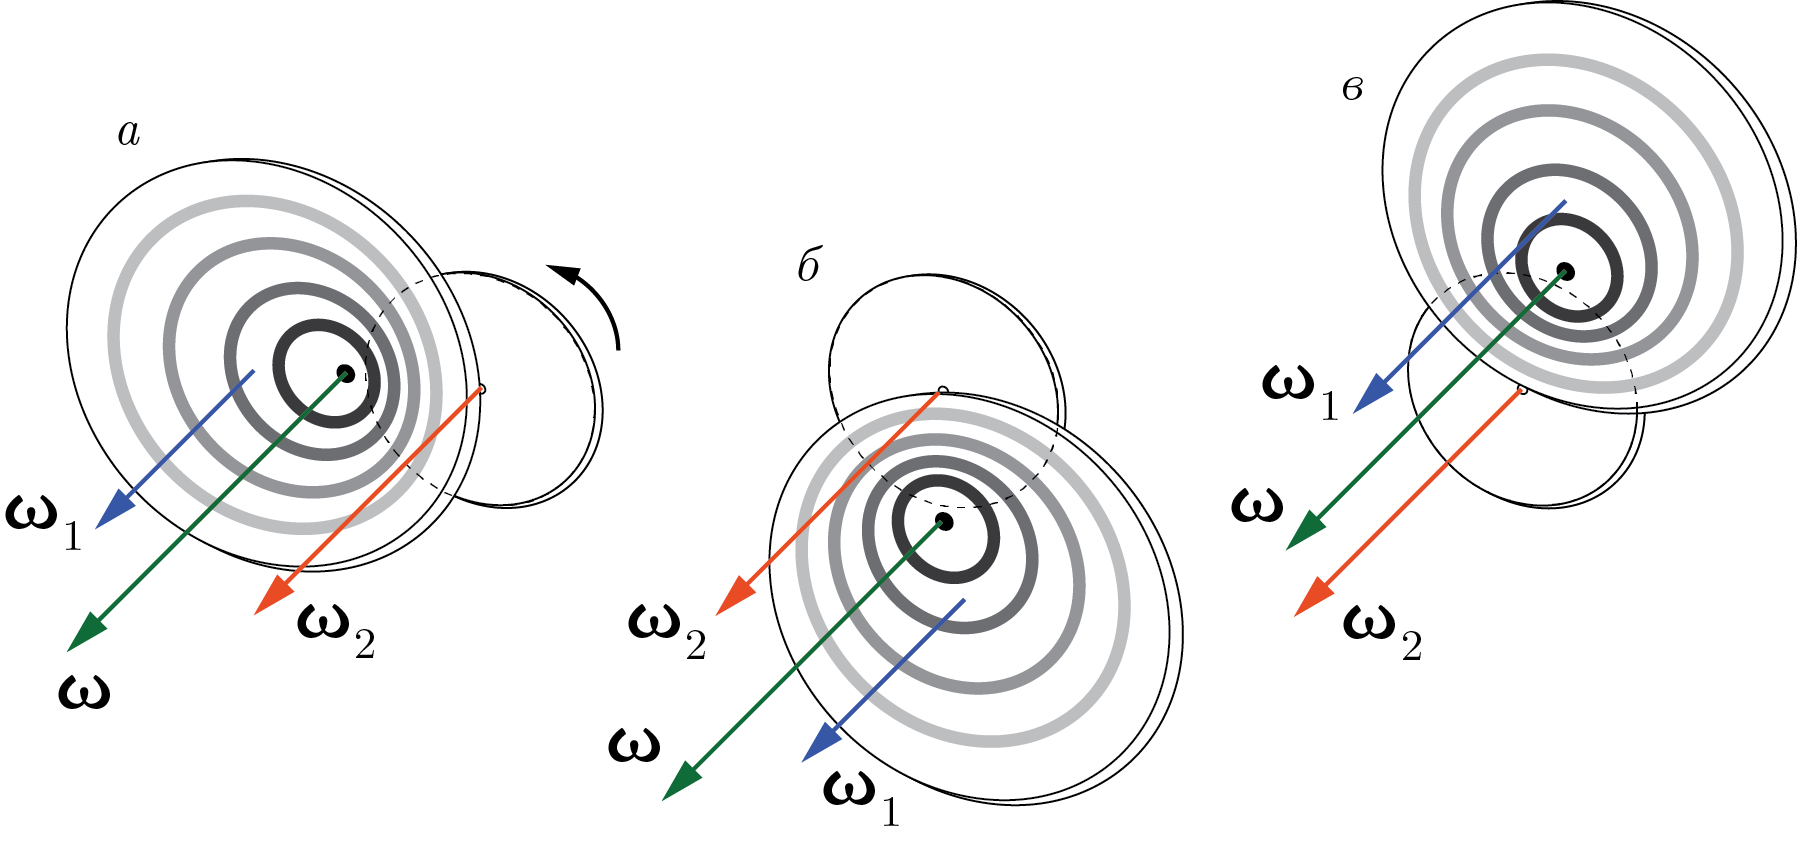
\includegraphics[width=0.9\linewidth]{aom-5.png}
	\caption{Вектор результирующей угловой скорости \textbf{ω} направлен вдоль мгновенной оси вращения, проходящей через точку на прямой, соединяющей центры диска и вала}
	\label{aom-5}
\end{figure}

Если угловые скорости $ \textbf{ω}_1$ и $ \textbf{ω}_2$ направлены в одну сторону (как показано на рис.\ref{aom-6}), то мгновенная ось вращения будет лежать на отрезке, соединяющем центры диска и вала. В противном случае, мгновенная ось вращения будет лежит за пределами этого отрезка. Положение мгновенной оси вращения можно определить через соотношение угловых скоростей:
$$
\dfrac{l_1}{l_2}  = \dfrac{\omega_2}{\omega_1},
$$
где через $ l_1 $ и $ l_2 $ обозначены расстояния от центра диска и вала до мгновенной оси (неразмытого пятна).

\begin{figure}[H]
	\centering 	
	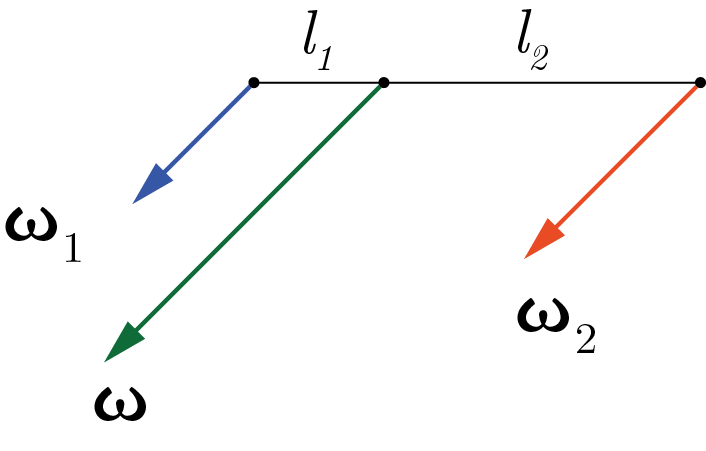
\includegraphics[width=0.3\linewidth]{aom-6.png}
	\caption{Векторы угловых скоростей диска и вала складываются, а направление результирующего вектора угловой скорости $\textbf{ω}$ совпадает с мгновенной осью вращения}
	\label{aom-6}
\end{figure}

Таким образом, по положению резкого пятна на вращающемся диске (рис.\ref{aom-3}) можно судить о соотношении угловых скоростей вращающихся тел. Чем больше собственная угловая скорость вращения диска по сравнению со скоростью вращения вала, там ближе мгновенная ось вращения расположена к оси диска. 

\end{document}